% DO NOT COMPILE THIS FILE DIRECTLY!
% This is included by the other .tex files.

\begin{frame}[t,plain]
\titlepage
\end{frame}

\begin{frame}
    \frametitle{\texttt{\$ whoami}}
    \begin{columns}
        \begin{column}{0.7\textwidth}
            \begin{itemize}
                \item Working @ circl.lu
                \item Part of the MISP-Project team
                \item Adding easter eggs for the past 4 years
            \end{itemize}
        \end{column}
        \begin{column}{0.3\textwidth}
            
\includegraphics[width=0.9\linewidth]{pictures/whoami.png}
        \end{column}
    \end{columns}
    \vspace*{0.75em}
    \begin{columns}
        \begin{column}{0.65\textwidth}
            \frame{
\includegraphics[width=1.0\linewidth]{pictures/whoami2.png}}
        \end{column}
        \begin{column}{0.35\textwidth}
            
\includegraphics[width=1.0\linewidth]{pictures/belgian-joke.jpeg}
        \end{column}
    \end{columns}
\end{frame}

\begin{frame}
    \frametitle{What problems are we trying to tackle?}
    \begin{itemize}
        \item \textbf{Prevent} default MISP behaviors to happen
        \item \textbf{Hook} specific actions to run callbacks
        \item Use-cases:
        \begin{itemize}
            \item Prevent publication of events not passing sanity checks
            \item Prevent querying thrid-party services with sensitive information
            \item Send notifications in a chat rooms
            \item And much much more...
        \end{itemize}
    \end{itemize}
\end{frame}

\begin{frame}
    \frametitle{What already exists in MISP?}
    
\includegraphics[width=16px]{pictures/python-logo.png}\hspace*{0.5em} \textbf{MISP API / PyMISP}
    \begin{itemize}
        \item Needs CRON Jobs in place
        \item Heavy for the server
        \item Not realtime
    \end{itemize}
    \vspace*{1em}
    
\includegraphics[width=16px]{pictures/zeromq.png}\hspace*{0.5em} \textbf{PubSub channels}
    \begin{itemize}
        \item After the actions happen: No feedback to MISP
        \item Tougher to put in place \& to share
        \item Full integration amounts to develop a new tool
    \end{itemize}
\end{frame}

\begin{frame}
    \frametitle{Simple automation made easy}
    \begin{center}
        
\includegraphics[width=0.3\linewidth]{pictures/automation.png}
    \end{center}
    \begin{itemize}
        \item Why?
        \begin{itemize}
            \item Everyone loves \textbf{simple automation}
            \item \textbf{Visual} dataflow programming
            \item Users want \textbf{more control}
        \end{itemize}
        \item How?
        \begin{itemize}
            \item \textbf{Drag \& Drop} editor
            \item Prevent actions \textbf{before they happen}
            \item Flexible \textbf{Plug \& Play} system
            \item \textbf{Share} workflows, \textbf{debug} and \textbf{replay}
        \end{itemize}
    \end{itemize}
\end{frame}

\begin{frame}
    \frametitle{Content of the presentation}
    \begin{itemize}
        \item MISP Workflows fundamentals
        \item Demo by examples
        \item Get started
        \item Using the system \& how it can be extended
    \end{itemize}

    \vspace*{1em}
    \begin{center}
        \frame{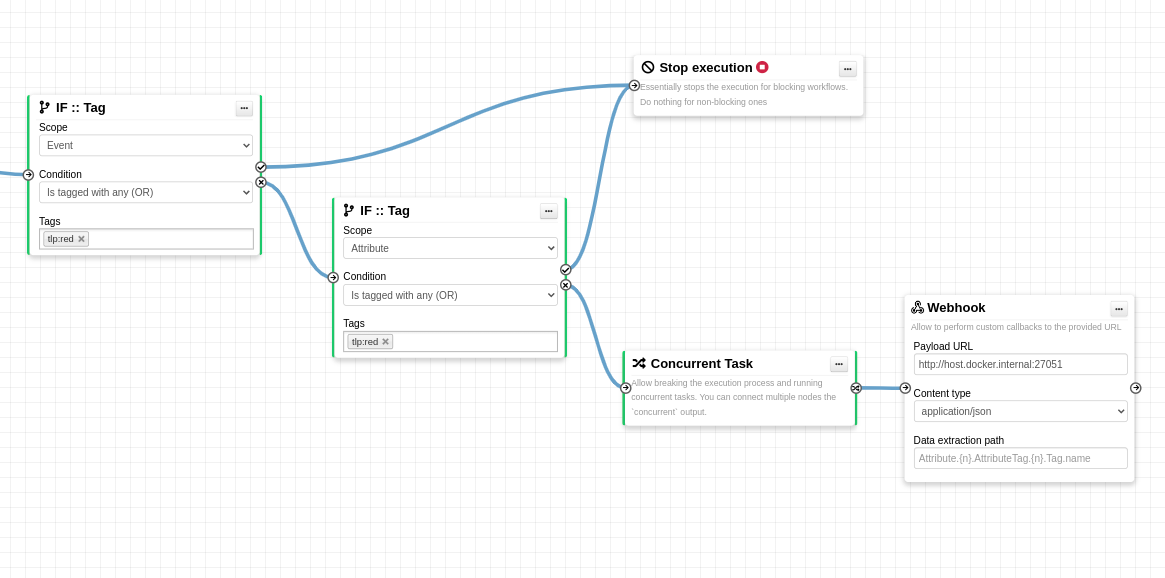
\includegraphics[width=0.7\linewidth]{pictures/overview.png}}
    \end{center}
\end{frame}

\section{Workflow - Fundamentals}
\begin{frame}
    \frametitle{How does it work}
    \begin{center}
        \frame{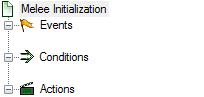
\includegraphics[width=0.4\linewidth]{pictures/event-condition-action.png}}
    \end{center}
    \begin{enumerate}
        \item An \textbf{event} happens in MISP
        \item Check if all \textbf{conditions} are satisfied
        \item Execute all \textbf{actions}
        \begin{itemize}
            \item May prevent MISP to complete its original event
        \end{itemize}
    \end{enumerate}
\end{frame}

\begin{frame}
    \frametitle{What kind of events?}
    
\includegraphics[width=60px]{pictures/sc-event.png}
    \vspace*{0.5em}
    \begin{itemize}
        \item New MISP Event
        \item Attribute has been saved
        \item New discussion post
        \item New user created
        \item Query against third-party services
        \item ...
    \end{itemize}
    \vspace*{1em}
    In MISP Workflow terminology, supported events are called \textbf{Triggers}
\end{frame}

\begin{frame}
    \frametitle{What kind of conditions?}
    
\includegraphics[width=70px]{pictures/sc-condition.png}
    \vspace*{0.5em}
    \begin{itemize}
        \item An MISP Event is tagged with \texttt{tlp:red}
        \item The distribution an Attribute is a sharing group
        \item The creator organisation is \texttt{circl.lu}
        \item Or any other \textbf{generic} conditions
    \end{itemize}

    \vspace*{1em}
    In MISP Workflow terminology, these are also called \textbf{Logic modules}
\end{frame}

\begin{frame}
    \frametitle{What kind of actions?}
    
\includegraphics[width=60px]{pictures/sc-action.png}
    \vspace*{0.5em}
    \begin{itemize}
        \item Send an email notification
        \item Perform enrichments
        \item Send a chat message on MS Teams
        \item Attach a local tag
        \item ...
    \end{itemize}

    \vspace*{1em}
    In MISP Workflow terminology, these are also called \textbf{Action modules}
\end{frame}

\begin{frame}
    \frametitle{What is a MISP Workflow?}
    \begin{itemize}
        \item Sequence of all nodes to be executed in the specified order
        \item Basically the whole connected graph.
        \item Workflows can be enabled / disabled
        \item Workflows are always linked to a \textbf{trigger}
    \end{itemize}
    \begin{center}
        \frame{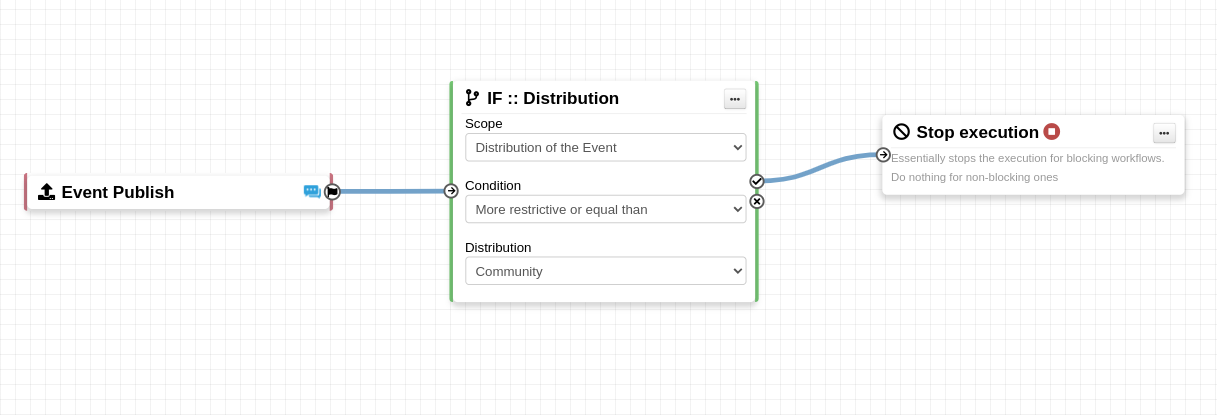
\includegraphics[width=1.0\linewidth]{pictures/simple-workflow.png}}
    \end{center}
\end{frame}

\begin{frame}
    \frametitle{Workflow execution for Event publish}
    \begin{itemize}
        \setlength\itemsep{1em}
        \item[] \hspace*{-2em}
\includegraphics[width=16px]{pictures/sc-event-icon.png} \hspace*{0.25em} An Event is about to be published
        \begin{itemize}
            \item The workflow for the \texttt{event-publish} trigger starts
        \end{itemize}
        \item[] \hspace*{-2em}
\includegraphics[width=16px]{pictures/sc-condition-icon.png} \hspace*{0.25em} Conditions are evaluated
        \item[] \hspace*{-2em}
\includegraphics[width=16px]{pictures/sc-action-icon.png} \hspace*{0.25em} Actions are executed
        \begin{itemize}
            \setlength\itemsep{0.75em}
            \item {\bf\color{green!50!black}success}: Continue the publishing action
            \hspace*{-4em}
\includegraphics[width=1.0\textwidth]{pictures/log-entry-publish-success.png}
            \item {\bf\color{red}failure} | \texttt{\color{red}blocked}: Stop publishing and log the reason
            \hspace*{-4em}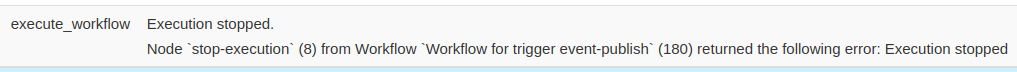
\includegraphics[width=1.0\textwidth]{pictures/log-entry-publish-blocked.png}
        \end{itemize}
    \end{itemize}
\end{frame}

\begin{frame}
    \frametitle{Blocking and non-blocking}
    Two types of workflows:
    \vspace{0.5em}
    \begin{itemize}
        \item[] \hspace*{-2em}
\includegraphics[width=48px]{pictures/blocking-workflow.png} Workflows
        \begin{itemize}
            \item Can prevent / block the original event to happen
            \item If a \textbf{blocking module}
\includegraphics[width=10px]{pictures/blocking-module.png} blocks the action
        \end{itemize}
        \vspace{0.5em}
        \item[] \hspace*{-2em}{\bf Regular} Workflows execution outcome has no impact
        \begin{itemize}
            \item \textbf{Blocking modules} No way to prevent something that has already happened
        \end{itemize}
        \begin{center}
            
\includegraphics[width=0.4\linewidth]{pictures/time-machine.png}
        \end{center}
    \end{itemize}
\end{frame}

\begin{frame}
    \frametitle{Workflow - Action modules}
    % \begin{center}
    %     
\includegraphics[width=0.6\linewidth]{pictures/module-type.png}
    % \end{center}
    \begin{itemize}
        \item 
\includegraphics[width=12px]{pictures/sc-action-icon.png} \textbf{action} modules: Allow to executes operations or custom scripts
        \begin{itemize}
            \item Tag operations
            \item Send notifications
            \item Webhooks
        \end{itemize}
    \end{itemize}
    \begin{center}
        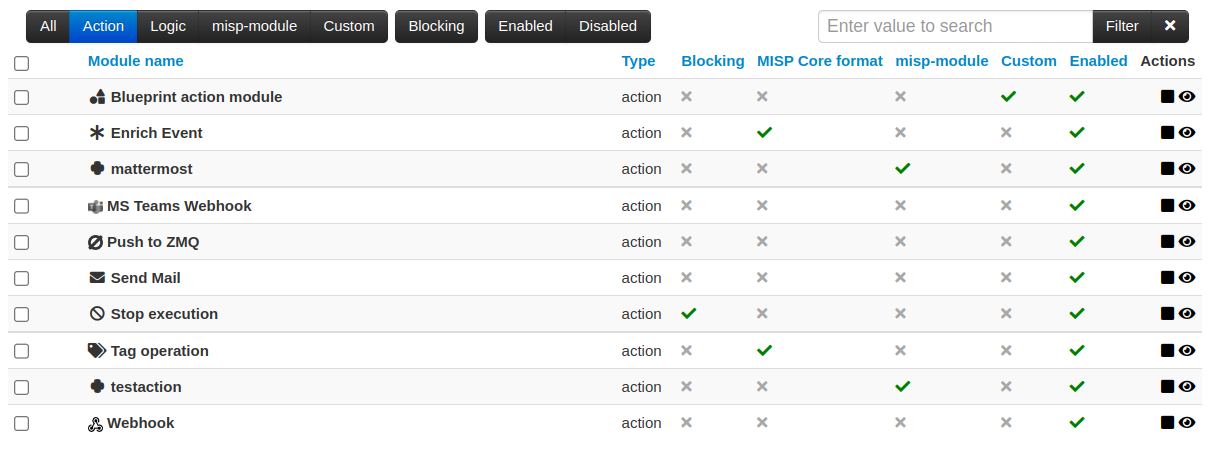
\includegraphics[width=1.0\linewidth]{pictures/action-module-index.png}
    \end{center}
\end{frame}

\begin{frame}
    \frametitle{Workflow - Logic modules}
    \begin{itemize}
        \item 
\includegraphics[width=12px]{pictures/sc-condition-icon.png} \textbf{logic} modules: Allow to redirect the execution flow.
        \begin{itemize}
            \item IF conditions
            \item Delay execution
        \end{itemize}
    \end{itemize}
    \begin{center}
        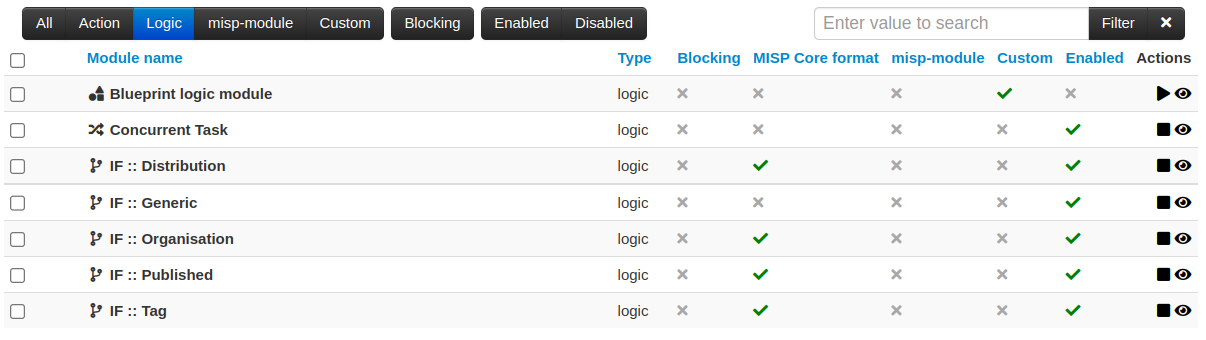
\includegraphics[width=1.0\linewidth]{pictures/logic-module-index.png}
    \end{center}
\end{frame}

\begin{frame}
    \frametitle{Sources of Workflow modules (1)}
    \begin{itemize}
        \item Built-in \textbf{default} modules
        \begin{itemize}
            \item Part of the MISP codebase
            \item Get in touch if you want us to increase the selection!
        \end{itemize}
    \end{itemize}
    \begin{center}
        
\includegraphics[width=1.0\linewidth]{pictures/module-buffet.png}
    \end{center}
\end{frame}

\begin{frame}
    \frametitle{Sources of Workflow modules (2)}
    User-defined \textbf{custom} modules
    \vspace*{0.5em}
    \begin{columns}
        \begin{column}{0.5\textwidth}
            \begin{itemize}
                \item Written in PHP
                \item Extend existing modules
                \item MISP code reuse
            \end{itemize}
        \end{column}
        \begin{column}{0.5\textwidth}
            
\includegraphics[width=1.0\linewidth]{pictures/php-joke.jpg}
        \end{column}
    \end{columns}
\end{frame}

\begin{frame}
    \frametitle{Sources of Workflow modules (3)}
    Modules from the 
\includegraphics[width=0.20\linewidth]{pictures/misp-module-icon.png} \textbf{enrichment service}
    \vspace*{0.5em}
    \begin{columns}
        \begin{column}{0.50\textwidth}
            \begin{itemize}
                \item Written in Python
                \item Can use any python libraries
                \item Plug \& Play
            \end{itemize}
        \end{column}
        \begin{column}{0.50\textwidth}
            
\includegraphics[width=1.0\linewidth]{pictures/python-joke.png}
        \end{column}
    \end{columns}
\end{frame}

\begin{frame}
    \frametitle{Triggers currently available}
    Currently 10 triggers can be hooked. 3 being 
\includegraphics[width=36px]{pictures/blocking-workflow.png}.
    \begin{center}
        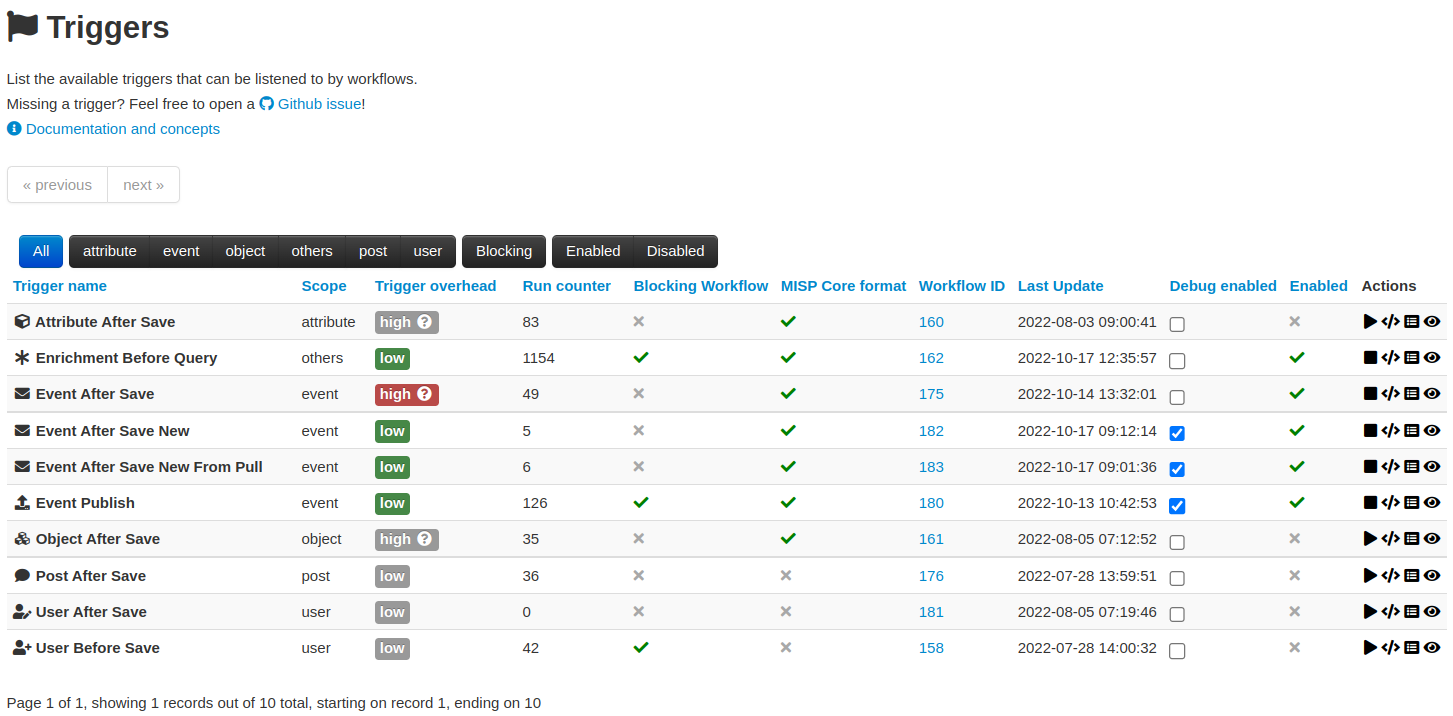
\includegraphics[width=1.0\linewidth]{pictures/triggers.png}
    \end{center}
\end{frame}

\begin{frame}
    \frametitle{Demo by examples}
    \begin{center}
        
\includegraphics[width=0.85\linewidth]{pictures/no-slides-if-demo.jpg}
    \end{center}
\end{frame}

\section{Workflow - Getting started}
\begin{frame}
    \frametitle{Getting started with workflows (1)}
    \begin{center}
        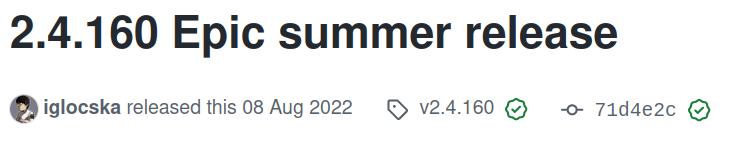
\includegraphics[width=0.9\linewidth]{pictures/workflow-release.png}
    \end{center}
    \begin{enumerate}
        \item Update your MISP server
        \item Update all your sub-modules
    \end{enumerate}
    \begin{center}
        
\includegraphics[width=0.6\textwidth]{pictures/upgrade-people.jpeg}
    \end{center}
\end{frame}

\begin{frame}
    \frametitle{Getting started with workflows (2)}
    Review MISP settings:
    \begin{enumerate}
        \item Make sure \texttt{\bf MISP.background\_jobs} is turned on
        \item Make sure workers are \textbf{up-and-running} and healthy
        \item Turn the setting \texttt{\bf Plugin.Workflow\_enable} on
    \end{enumerate}
    \begin{center}
        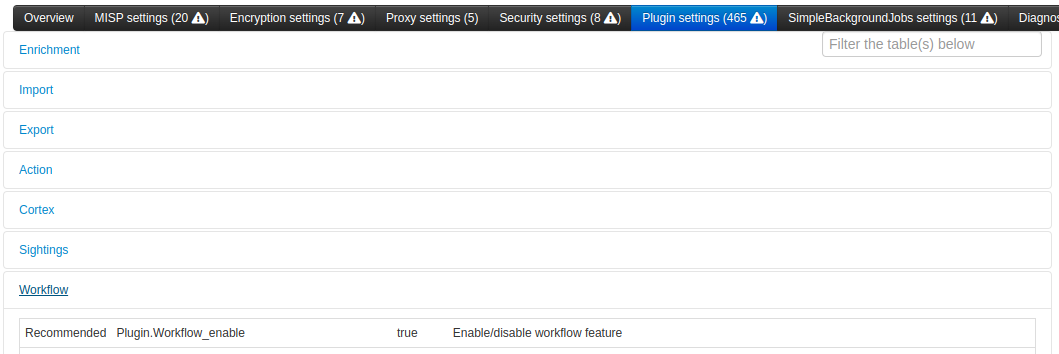
\includegraphics[width=1.0\textwidth]{pictures/settings-2.png}
    \end{center}
\end{frame}

\begin{frame}
    \frametitle{Getting started with workflows (3)}
    [optional] Wanna enjoy 
\includegraphics[width=0.17\linewidth]{pictures/misp-module-icon.png} ?
    \begin{enumerate}
        \item Turn the setting \texttt{\bf Plugin.Action\_services\_enable} on
    \end{enumerate}
    \begin{center}
        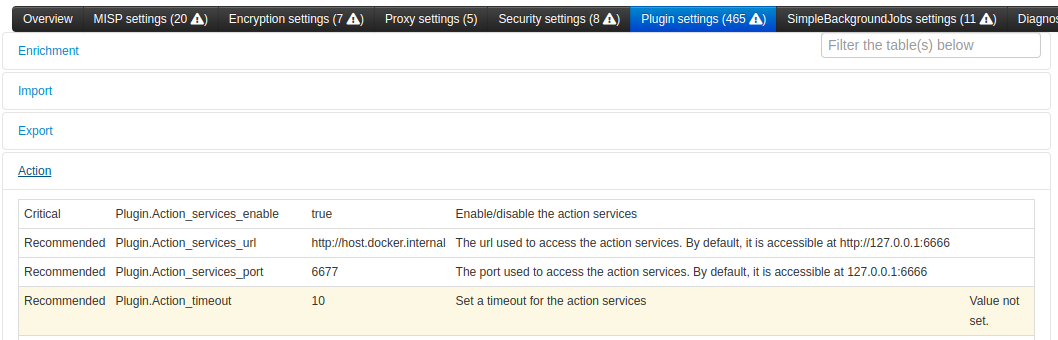
\includegraphics[width=1.0\textwidth]{pictures/settings-1.png}
    \end{center}
\end{frame}

\begin{frame}
    \frametitle{Getting started with workflows (4)}
    \begin{enumerate}
        \item Go to the list of modules
        \begin{itemize}
            \item \texttt{Administration > Workflows > List Modules}
            \item or \url{/workflows/moduleIndex}
        \end{itemize}
        \item Make sure \textbf{default} modules are loaded
        \item {[optional:misp-module]} Make sure \textbf{misp-module} modules are loaded
    \end{enumerate}
\end{frame}

\begin{frame}
    \frametitle{Getting started with workflows (4)}
    \centering
    {\Large Everything is ready?}\\
    \vspace*{3em}
    {\LARGE Let's see how to build a workflow!}
\end{frame}

\begin{frame}
    \frametitle{Creating a workflow with the editor}
    \begin{center}
        \begin{tikzpicture}
            \node[align=left] (img1) at (0, 0) {
                $\blacktriangleright$ 1. Go to the list of triggers \texttt{Administration > Workflows} \\
                $\blacktriangleright$ 2. Enable the trigger \\
                $\blacktriangleright$ 3. Edit the \texttt{trigger} you want to create a workflow for \\
                $\blacktriangleright$ 4. Drag an \texttt{action} module from the side panel\\
                to the canvas \\
                $\blacktriangleright$ 5. Drag another \texttt{action} module or a logic module\\
                from the side panel to the canvas \\
                $\blacktriangleright$ 6. From the \texttt{trigger} output, drag an arrow into\\
                the \texttt{action}'s input (left side) \\
                $\blacktriangleright$ 7. Continue linking modules with the input/output system\\
                until all wanted modules are connected \\
                $\blacktriangleright$ 8. Find an action that would execute the desired trigger \\
                $\blacktriangleright$ 9. Execute the action and observe the effect! \\
                $\blacktriangleright$ 10. Optionally, enable debug mode to see realtime execution \\
                $\blacktriangleright$ 10.1. Even more text to make the slide even more unreadable \\
                $\blacktriangleright$ 10.2. And even more boring
            };
            \pause
            \node (img2) at (0, 0) {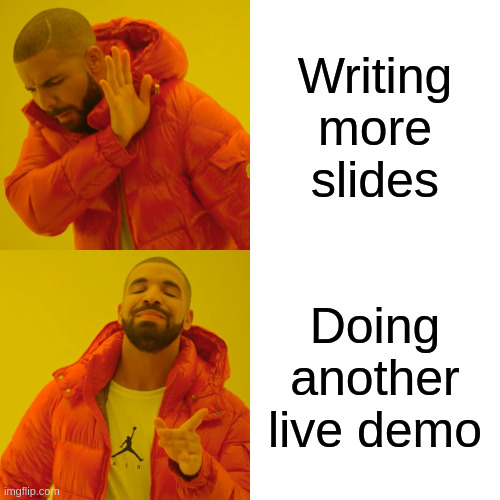
\includegraphics[width=0.6\textwidth]{pictures/no-slides-if-demo3.jpg}};
        \end{tikzpicture}
    \end{center}
\end{frame}

\section{Considerations when working with workflows}
\begin{frame}
    \frametitle{Working with the editor - Operations not allowed}
    Execution loop are not authorized
    \vspace*{1em}
    \begin{columns}
        \begin{column}{0.7\textwidth}
            \frame{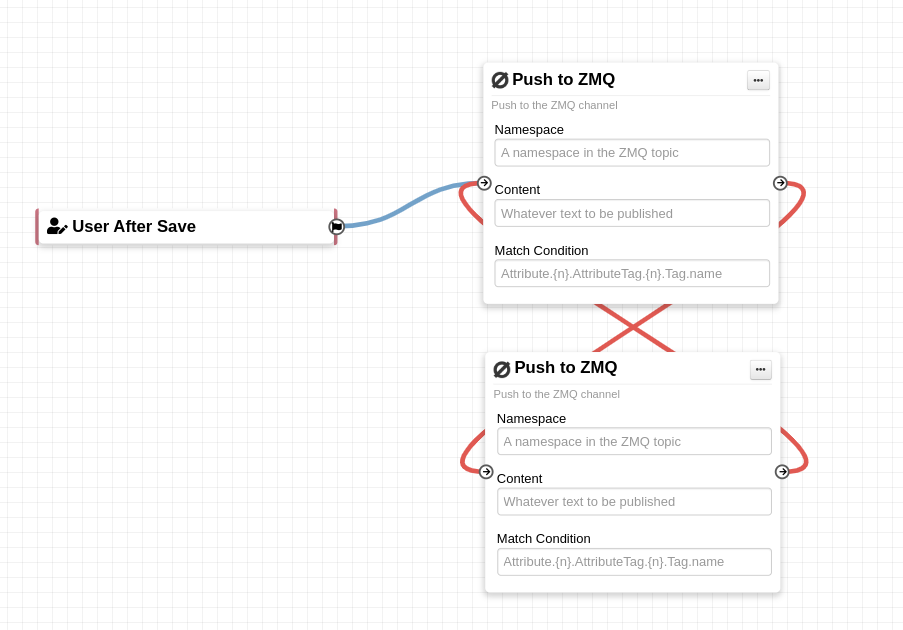
\includegraphics[width=1.0\linewidth]{pictures/editor-not-allowed-1.png}}
        \end{column}
        \begin{column}{0.3\textwidth}
            \frame{
\includegraphics[width=1.0\linewidth]{pictures/infinite-loop.jpg}}
        \end{column}
    \end{columns}
\end{frame}

\begin{frame}
    \frametitle{Recursive workflows}
    \frame{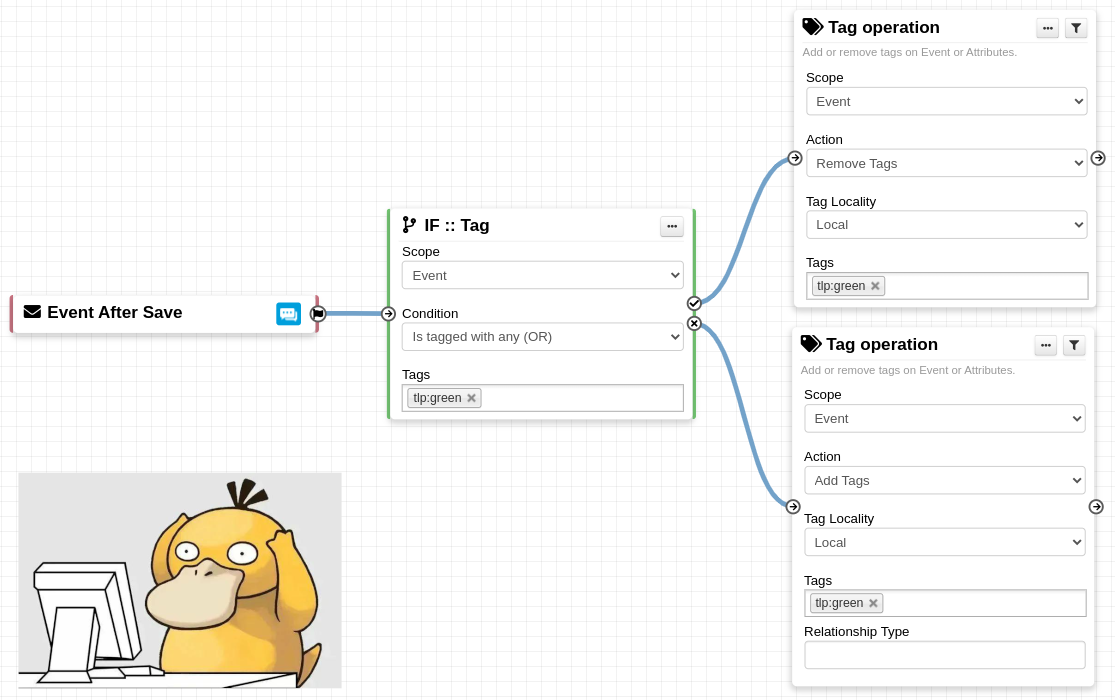
\includegraphics[width=1.0\linewidth]{pictures/recursive-workflow.png}}
    \danger Recursion: If an action re-run the workflow
\end{frame}

\begin{frame}
    \frametitle{Working with the editor - Operations not allowed}
    Multiple connections from the same output
    \vspace*{1em}
    \begin{columns}
        \begin{column}{0.7\textwidth}
            \frame{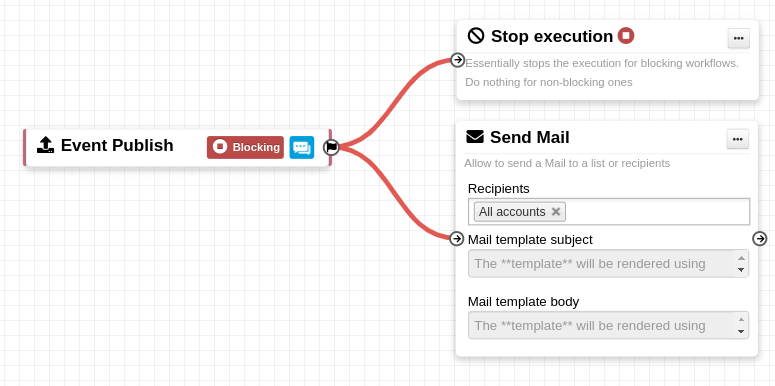
\includegraphics[width=1.0\linewidth]{pictures/editor-not-allowed-2.png}}
        \end{column}
        \begin{column}{0.3\textwidth}
            \frame{
\includegraphics[width=1.0\linewidth]{pictures/two-paths.jpeg}}
        \end{column}
    \end{columns}
    \begin{itemize}
        \item Execution order not guaranted
        \item Confusing for users
    \end{itemize}
\end{frame}

\begin{frame}
    \frametitle{Working with the editor}
    Cases showing a warning:
    \begin{itemize}
        \item \textbf{Blocking} modules 
\includegraphics[width=10px]{pictures/blocking-module.png} in a \textbf{non-blocking} workflow 
\includegraphics[width=0.12\linewidth]{pictures/time-machine.png}
        \item \textbf{Blocking} modules 
\includegraphics[width=10px]{pictures/blocking-module.png} after a \textbf{concurrent tasks} module
        \begin{center}
            \frame{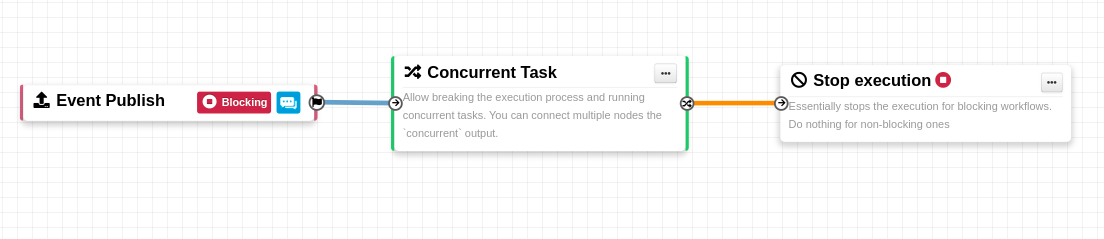
\includegraphics[width=1.0\linewidth]{pictures/editor-warning-1.png}}
        \end{center}
    \end{itemize}
\end{frame}

\section{Advanced usage}
\begin{frame}
    \frametitle{Workflow blueprints}
    \hspace*{0.9\textwidth}
\includegraphics[width=32px]{pictures/blueprint-32.png}
    \vspace*{-2em}
    \begin{enumerate}
        \item Blueprints allow to \textbf{re-use parts} of a workflow in another one
        \item Blueprints can be saved, exported and \textbf{shared}
    \end{enumerate}
    \begin{center}
        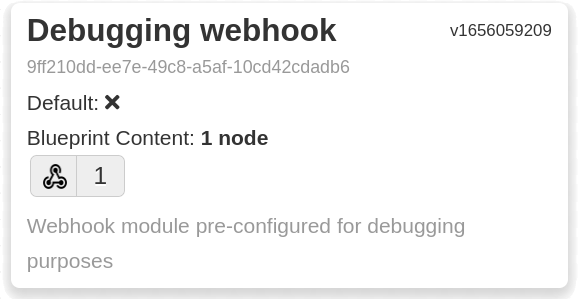
\includegraphics[width=0.5\linewidth]{pictures/blueprint-debugging.png}
    \end{center}
    Blueprints sources:
    \begin{enumerate}
        \item Created or imported by users
        \item From the \texttt{MISP/misp-workflow-blueprints} repository\footnote{\scriptsize https://github.com/MISP/misp-workflow-blueprints}
    \end{enumerate}
\end{frame}

\begin{frame}[fragile]
    \frametitle{Hash path filtering}
Filtering and checking conditions using hash path expression.
\begin{lstlisting}[language=javascript,firstnumber=1]
$path_expression = '{n}[name=fred].id';
$users = [
    {'id': 123, 'name': 'fred', 'surname': 'bloggs'},
    {'id': 245, 'name': 'fred', 'surname': 'smith'},
    {'id': 356, 'name': 'joe', 'surname': 'smith'},
];
$ids = Hash::extract($users, $path_expression);
// => $ids will be [123, 245]
\end{lstlisting}
\begin{columns}
    \begin{column}{0.6\textwidth}
        \begin{center}
            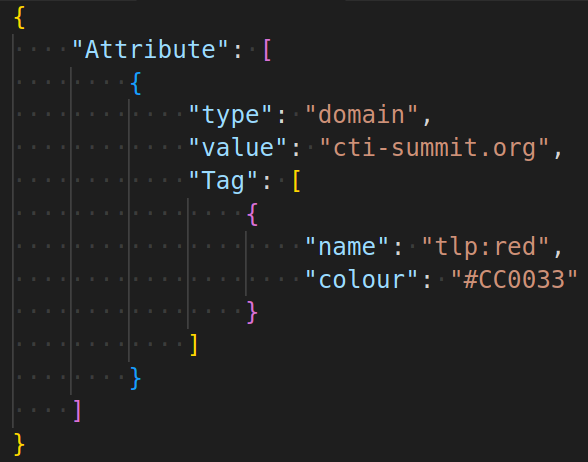
\includegraphics[width=0.7\linewidth]{pictures/attribute-json.png}
        \end{center}
    \end{column}
    \begin{column}{0.4\textwidth}
        \includegraphics[width=1.0\linewidth]{pictures/module-if-generic.png}
    \end{column}
\end{columns}
\end{frame}

\begin{frame}
    \frametitle{Data format in Workflows}
    \begin{center}
        \includegraphics[width=0.7\linewidth]{pictures/workflow-trigger.png}
    \end{center}
    \begin{itemize}
        \item In most cases, the format is compliant with the \textbf{MISP Core format}
        \item But data has \textbf{additional properties}
        \begin{itemize}
            \item Attributes are \textbf{always encapsulated} in the Event or Object
            \item Additional key \textbf{\texttt{\_AttributeFlattened}}
            \item Additional key \textbf{\texttt{\_allTags}}
            \item Additional key \textbf{\texttt{inherited}} for Tags
        \end{itemize}
    \end{itemize}
\end{frame}

\begin{frame}
    \frametitle{Logic module: Concurrent Task}
    \begin{itemize}
        \item Logic module allowing \textbf{multiple output} connections
        \item \textbf{Postpone the execution} for remaining modules
        \item Blocking modules\includegraphics[width=10px]{pictures/blocking-module.png} \textbf{cannot cancel} ongoing operations \includegraphics[width=0.05\linewidth]{pictures/time-machine.png}
    \end{itemize}
    \begin{center}
        \frame{\includegraphics[width=0.5\linewidth]{pictures/module-concurrent.png}}
    \end{center}
\end{frame}

\section{Debugging}
\begin{frame}
    \frametitle{Debugging Workflows: Log Entries}
    \begin{itemize}
        \item Workflow execution is logged in the application logs:
        \begin{itemize}
            \item \texttt{/admin/logs/index}
        \end{itemize}
        \item Or stored on disk in the following file:
        \begin{itemize}
            \item \texttt{/app/tmp/logs/workflow-execution.log}
        \end{itemize}
    \end{itemize}
    \begin{center}
        \includegraphics[width=1.0\linewidth]{pictures/workflow-debug.png}
    \end{center}
\end{frame}

\begin{frame}
    \frametitle{Debugging Workflows: Debug mode}
    \begin{itemize}
        \item The \includegraphics[width=70px]{pictures/debug-mode.png} can be turned on for each workflows
        \item Each nodes will send data to the provided URL
        \begin{itemize}
            \item Configure the setting: \texttt{Plugin.Workflow\_debug\_url}
        \end{itemize}
        \item Result can be visualized in
        \begin{itemize}
            \item \textbf{offline}: \texttt{tools/misp-workflows/webhook-listener.py}
            \item \textbf{online}: \url{requestbin.com} or similar websites
        \end{itemize}
    \end{itemize}
    \begin{center}
        \includegraphics[width=0.6\linewidth]{pictures/request-bin.png}
    \end{center}
\end{frame}

\begin{frame}
    \frametitle{Debugging modules: Stateless execution}
    \begin{itemize}
        \item Test custom modules with custom input
    \end{itemize}
    \begin{center}
        \includegraphics[width=1.0\linewidth]{pictures/stateless-execution.png}
    \end{center}
\end{frame}

\begin{frame}
    \frametitle{Debugging modules: Re-running workflows}
    \begin{itemize}
        \item Try workflows with custom input
        \item Re-run workflows to ease debugging
    \end{itemize}
    \begin{center}
        \frame{\includegraphics[width=0.55\linewidth]{pictures/running-workflows.png}}
    \end{center}
\end{frame}

\begin{frame}
    \frametitle{Debugging options}
    \begin{columns}
        \begin{column}{0.6\textwidth}
            \begin{itemize}
                \item Workflow execution and outcome
                \item Module execution and outcome
                \item Live workflow debugging with module inspection
                \item Re-running/testing workflows with custom data
                \item Stateless module execution
            \end{itemize}
        \end{column}
        \begin{column}{0.4\textwidth}
            \includegraphics[width=1.0\linewidth]{pictures/enough-debugging.jpg}
        \end{column}
    \end{columns}
\end{frame}

\section{Extending the system}
\begin{frame}
    \frametitle{Creating a new module in PHP}
    \begin{center}
        \includegraphics[width=0.65\linewidth]{pictures/custom-1.png}
    \end{center}

    \begin{itemize}
        \item \texttt{\small \textbf{app/Lib/}WorkflowModules/action/[module\_name].php}
        \item Designed to be easilty extended
        \begin{itemize}
            \item Helper functions
            \item Module configuration as variables
            \item Implement runtime logic
        \end{itemize}
    \end{itemize}
\end{frame}

\begin{frame}
    \frametitle{Creating a new module in Python}
    \begin{center}
        \includegraphics[width=0.65\linewidth]{pictures/custom-2.png}
    \end{center}

    \begin{itemize}
        \item Similar to how other \texttt{misp-modules} are implemented
        \begin{itemize}
            \item Helper functions
            \item Module configuration as variables
            \item Implement runtime logic
        \end{itemize}
    \end{itemize}
\end{frame}

\begin{frame}
    \frametitle{Ideas}
    \begin{itemize}
        \item Chat notification a community when new user joins an instance
        \item Trigger on any action via log entries
        \item Extend existing MISP behavior: Push correlation in another system
        \item Sanity check to block publishing
        \item ...
    \end{itemize}
\end{frame}

\begin{frame}
    \frametitle{Future works}
    \begin{columns}
        \begin{column}{0.55\textwidth}
            \begin{itemize}
                \item More \includegraphics[width=12px]{pictures/sc-action-icon.png} modules
                \item More \includegraphics[width=12px]{pictures/sc-condition-icon.png} modules
                \item More \includegraphics[width=12px]{pictures/sc-event-icon.png} triggers
                \item More documentation
                \item Recursion prevention system
                \item On-the-fly data override?
            \end{itemize}
        \end{column}
        \begin{column}{0.45\textwidth}
            \includegraphics[width=1.0\linewidth]{pictures/future-works.jpeg}
        \end{column}
    \end{columns}
\end{frame}

\begin{frame}
    \frametitle{Final words}
    \begin{columns}
        \begin{column}{0.6\textwidth}
            \begin{itemize}
                \item Feature designed to quickly and cheaply support CTI pipeline
                \item \textbf{Beta}: Feature unlikely to change. But still..
                \item Waiting for feedback!
            \end{itemize}
        \end{column}
        \begin{column}{0.4\textwidth}
            \includegraphics[width=1.0\linewidth]{pictures/feeling-of-power.jpg}
        \end{column}
    \end{columns}
    \vspace*{0.5em}
    \includegraphics[width=1.0\linewidth]{pictures/first-cti.png}
\end{frame}

